\documentclass{beamer}

%\usepackage{t1enc}
%\pgfpagelayout{2 on 1}[a4paper]

\usepackage{beamerthemesplit,bm}
\usepackage[latin1]{inputenc}
\usepackage[italian]{babel}
\usepackage{graphicx}
% \usepackage{movie15}
\usepackage{hyperref}
\usepackage{multimedia}
\usepackage{subfigure}
\usepackage{xcolor}
\usepackage{amsmath,amssymb}
\usepackage{stmaryrd}

\usetheme{Boadilla}


\definecolor{mygreen}{rgb}{0,0.48,0.0}

\definecolor{myblue}{rgb}{0,0,0.64}

\author{Alessio Fumagalli}
\date{08-10-2010}
\institute{Politecnico di Milano}

\begin{document}

%---------------------------------------------------------------------------------

\begin{frame}

	\frametitle{Gnuplot}	
	
	\begin{block}{Introduzione a}
		\centering
		Gnuplot
	\end{block}

	\vspace{1cm}

	\begin{block}{Pagine web utili}
		\centering
		\begin{itemize}
			\item http://www.gnuplot.info/
			\item http://t16web.lanl.gov/Kawano/gnuplot/legend-e.html
		\end{itemize}
	\end{block}

\end{frame}

%---------------------------------------------------------------------------------

\begin{frame}
	
	\frametitle{Gnuplot}

	\begin{block}{Gnuplot}
		\centering
		Gnuplot � un utility, a linea di comando, per visualizzare funzioni matematiche e dati in modo interattivo.
	\end{block}

	\vspace{1cm}	
	
	\begin{block}{}
		� anche utilizzato come libreria grafica in molte applicazioni, ad esempio Octave.
	\end{block}

\end{frame}

%---------------------------------------------------------------------------------

\begin{frame}

	\frametitle{Gnuplot}
	
	\begin{block}{Esempi}
	
		\centering
		
		\begin{minipage}{0.5\textwidth}
			\centering
			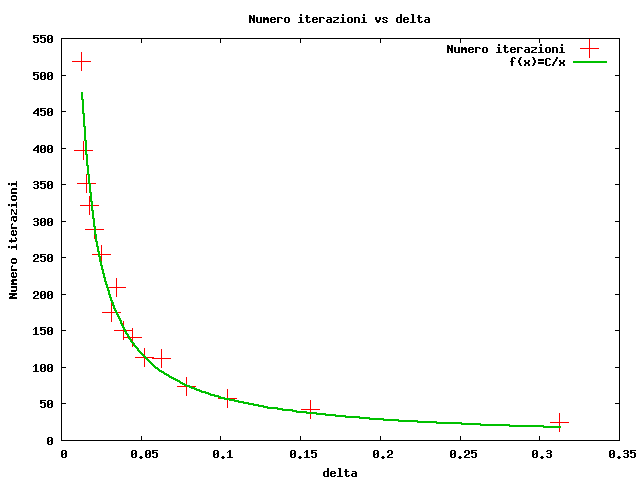
\includegraphics[width=0.95\textwidth]{images/iter_vs_delta}
		\end{minipage}%
		\begin{minipage}{0.5\textwidth}
			\centering
			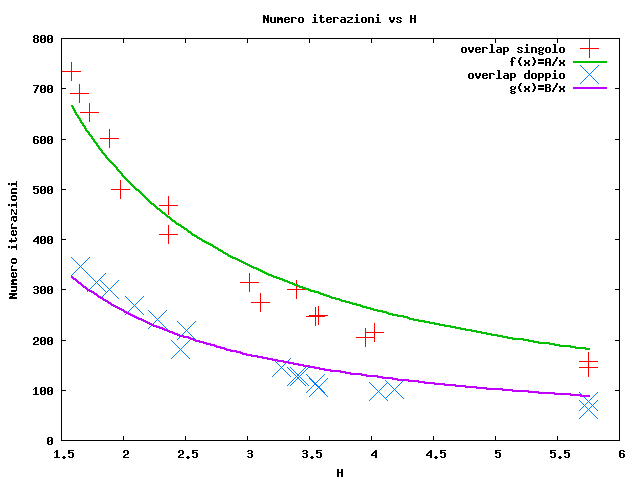
\includegraphics[width=0.95\textwidth]{images/iter_vs_H}
		\end{minipage}
		
	\end{block}

\end{frame}

%---------------------------------------------------------------------------------

\begin{frame}

	\frametitle{Gnuplot}
	
	\begin{block}{Esempi}
	
		\centering
		
		\begin{minipage}{0.5\textwidth}
			\centering
			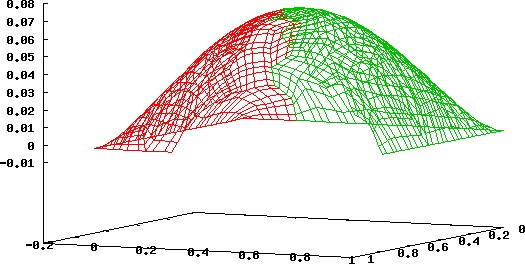
\includegraphics[width=0.95\textwidth]{images/img1}
		\end{minipage}%
		\begin{minipage}{0.5\textwidth}
			\centering
			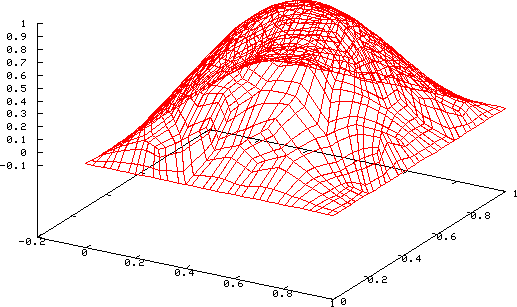
\includegraphics[width=0.95\textwidth]{images/soluzione2}
		\end{minipage}
		
	\end{block}

\end{frame}

%---------------------------------------------------------------------------------

\begin{frame}[fragile]

	\frametitle{Gnuplot}

	\begin{block}{Comandi utilizzati per l'ultimo grafico}	
		\begin{verbatim}
		set terminal png
		set key off
		set output "soluzione/soluzione.png"
		splot "soluzione/soluzione.dat" with lines
		\end{verbatim}
	\end{block}

	\vspace{1cm}
	
	\begin{block}{ }
		La gran parte della difficolt\`a in Gnuplot \`e salvare in maniera corretta i dati che verranno utilizzati per la visualizzazione.
	\end{block}

\end{frame}

%---------------------------------------------------------------------------------

\begin{frame}[fragile]

	\frametitle{Gnuplot}
	
	\begin{block}{Problema}
		Dato il file \verb1data1 visualizzare le curve corrispondenti.
	\end{block}
	
	\begin{block}{data}
		\begin{verbatim}
			#   X         Y1         Y2         Y3
   -1.0000    0.0000     0.0000     1.0000
   -0.9000    0.5700     1.1769     0.7150
   -0.8000    1.0800     1.4400     0.4600
   -0.7000    1.5300     1.4997     0.2350
   -0.6000    1.9200     1.4400     0.0400
   -0.5000    2.2500     1.2990    -0.1250
   -0.4000    2.5200     1.0998    -0.2600
   -0.3000    2.7300     0.8585    -0.3650
   -0.2000    2.8800     0.5879    -0.4400
   -0.1000    2.9700     0.2985    -0.4850
    0.0000    3.0000    -0.0000    -0.5000
    0.1000    2.9700    -0.2985    -0.4850
    0.2000    2.8800    -0.5879    -0.4400
    0.3000    2.7300    -0.8585    -0.3650
    0.4000    2.5200    -1.0998    -0.2600
    0.5000    2.2500    -1.2990    -0.1250
    0.6000    1.9200    -1.4400     0.0400
    0.7000    1.5300    -1.4997     0.2350
    0.8000    1.0800    -1.4400     0.4600
    0.9000    0.5700    -1.1769     0.7150
    1.0000    0.0000    -0.0000     1.0000

		\end{verbatim}
	\end{block}

\end{frame}

%---------------------------------------------------------------------------------

\begin{frame}[fragile]

	\frametitle{Gnuplot}

	\begin{block}{Comandi Gnuplot}
		\begin{verbatim}
			plot "data" using 1:2 with lines,\
			     "data" using 1:3 with lines,\
			     "data" using 1:4 with lines
		\end{verbatim}		
	\end{block}	

	\begin{figure}[!h]
		\centering
		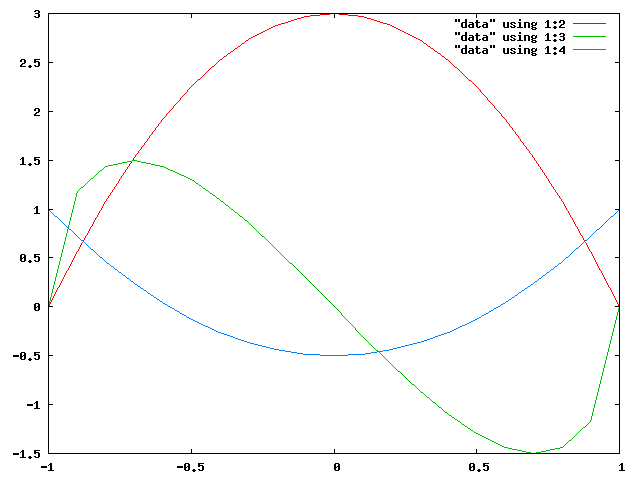
\includegraphics[width=0.5\textwidth]{images/graph}
	\end{figure}
	
\end{frame}

%---------------------------------------------------------------------------------

\begin{frame}[fragile]
	
	\frametitle{Gnuplot}

	\begin{block}{Comandi per salvare l'output, da anteporre al plot}		
		
		\begin{verbatim}
		set terminal png
		set output "graph.png"
		\end{verbatim}		
		
	\end{block}
	
	\vspace{1cm}
	
	\begin{block}{}
		Vi sono numerosi formati di output disponibili: png, fig, pslatex, svg, \ldots
	\end{block}

	\vspace{1cm}	
	
	\begin{block}{Per tornare alla visualizzazione a schermo}
	
		\begin{verbatim}
		set terminal x11		
		\end{verbatim}
		
	\end{block}
	
\end{frame}

%---------------------------------------------------------------------------------

\begin{frame}[fragile]
	
	\frametitle{Gnuplot}
	
	\begin{block}{ }
		\`E possibile far eseguire a Gnuplot degli script di comandi salvati su file.
		
		\begin{verbatim}
		gnuplot file_comandi
		\end{verbatim}	
		
	\end{block}
	
	\vspace{1cm}
	
	\begin{block}{C++}
		All'interno di un programma C++ \`e possibile invocare Gnuplot attraverso il comando \texttt{system} contenuto in \texttt{cstdlib}
		
		\begin{verbatim}
			system("gnuplot file_comandi");
		\end{verbatim}

		In realt\`a il comando \texttt{system} permette di eseguire ogni comando del sistema operativo.
	\end{block}	

\end{frame}

\end{document}